\chapter{Présentation du sujet}
\label{presentation_sujet}

\section{Objectifs}

\paragraph{}
Le but du projet a été de continuer le travail entrepris via la première
version de l'application afin d'obtenir trois niveaux de vues (atome, molécule
et réaction), un design en agents et des mouvements d'atomes plus réalistes qui
sont soumis à des lois d'attraction/répulsion


\section{Aperçus}

\paragraph{}
Voici différents aperçus de l'application réalisée :

\begin{figure}[H]
\centering
\centerline{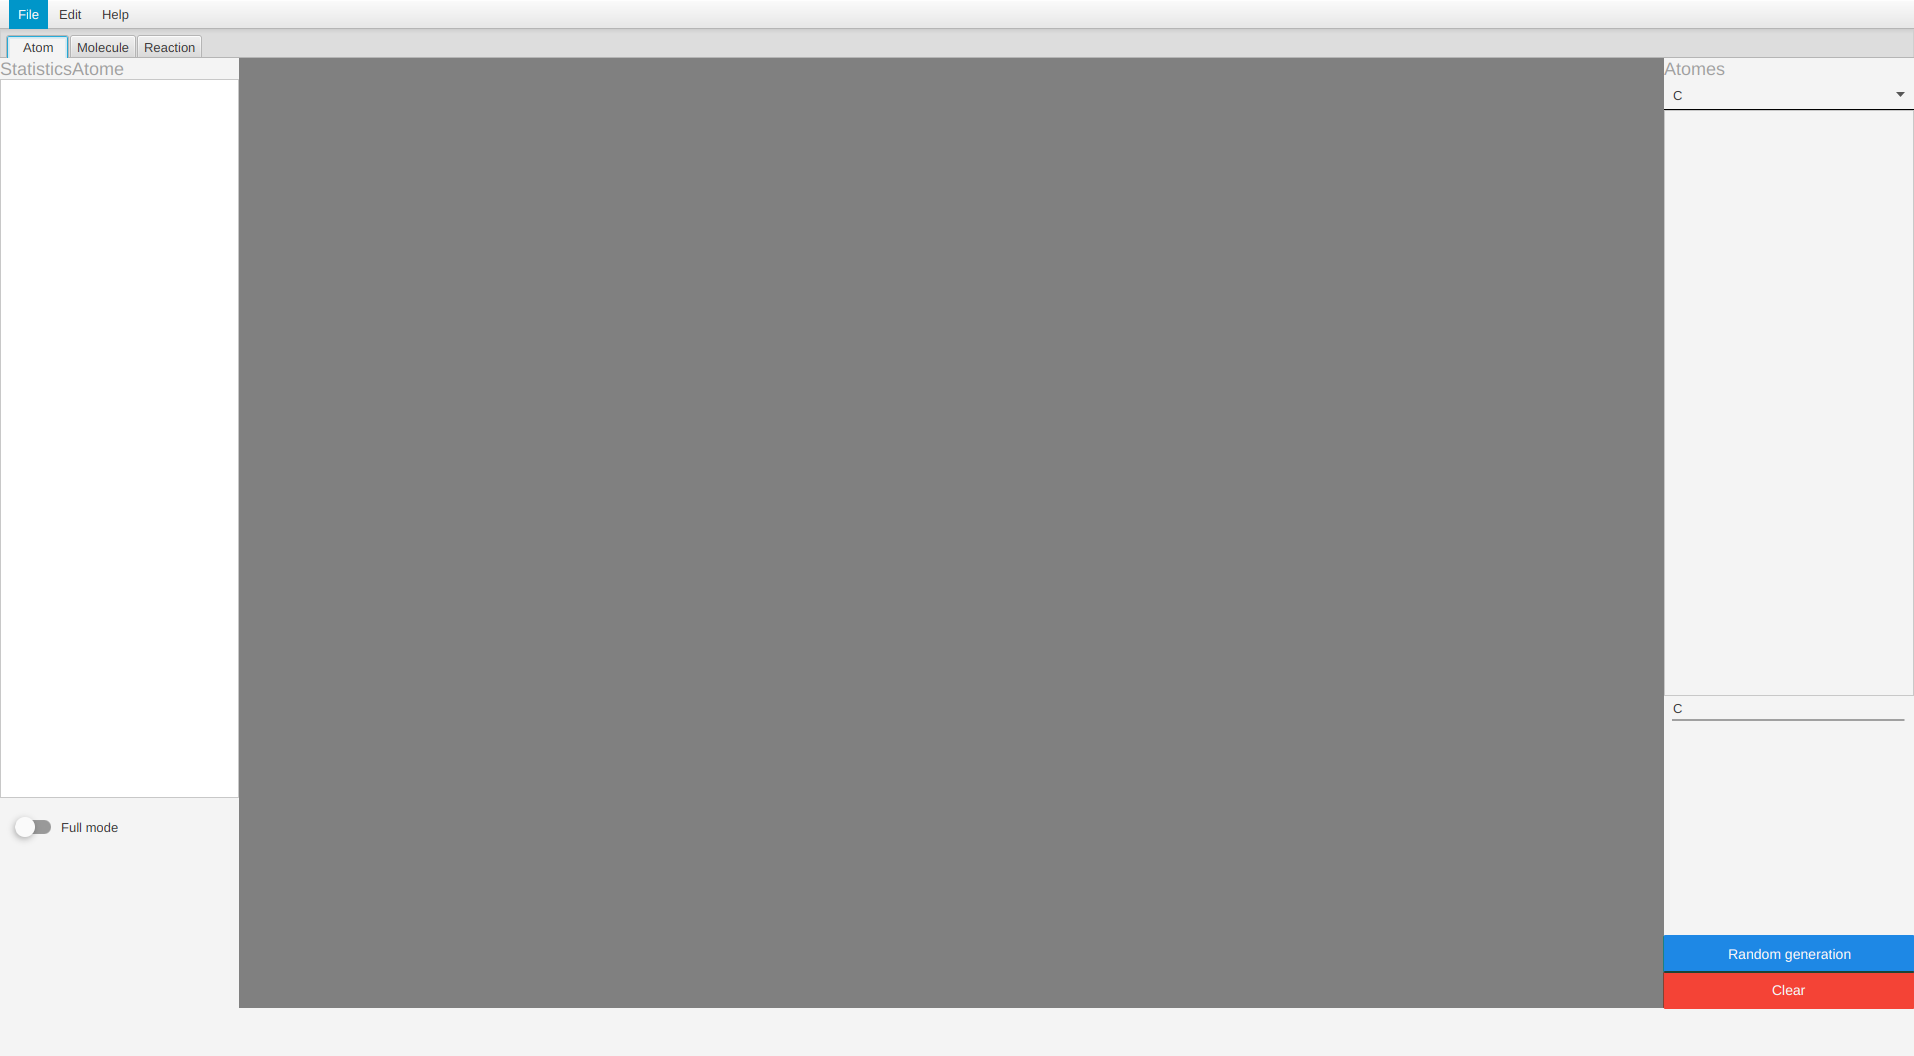
\includegraphics[width=1.2\textwidth]{screenshot_atom}}
\caption{Vue sur l'onglet Atome}
\label{screenshot_atom}
\end{figure}

\paragraph{}
La vue Atome permet normalement de générer un atome et de le visualiser.
Cependant, à la fin de cette TX, il n'est pas encore fonctionnel.

\begin{figure}[H]
\centering
\centerline{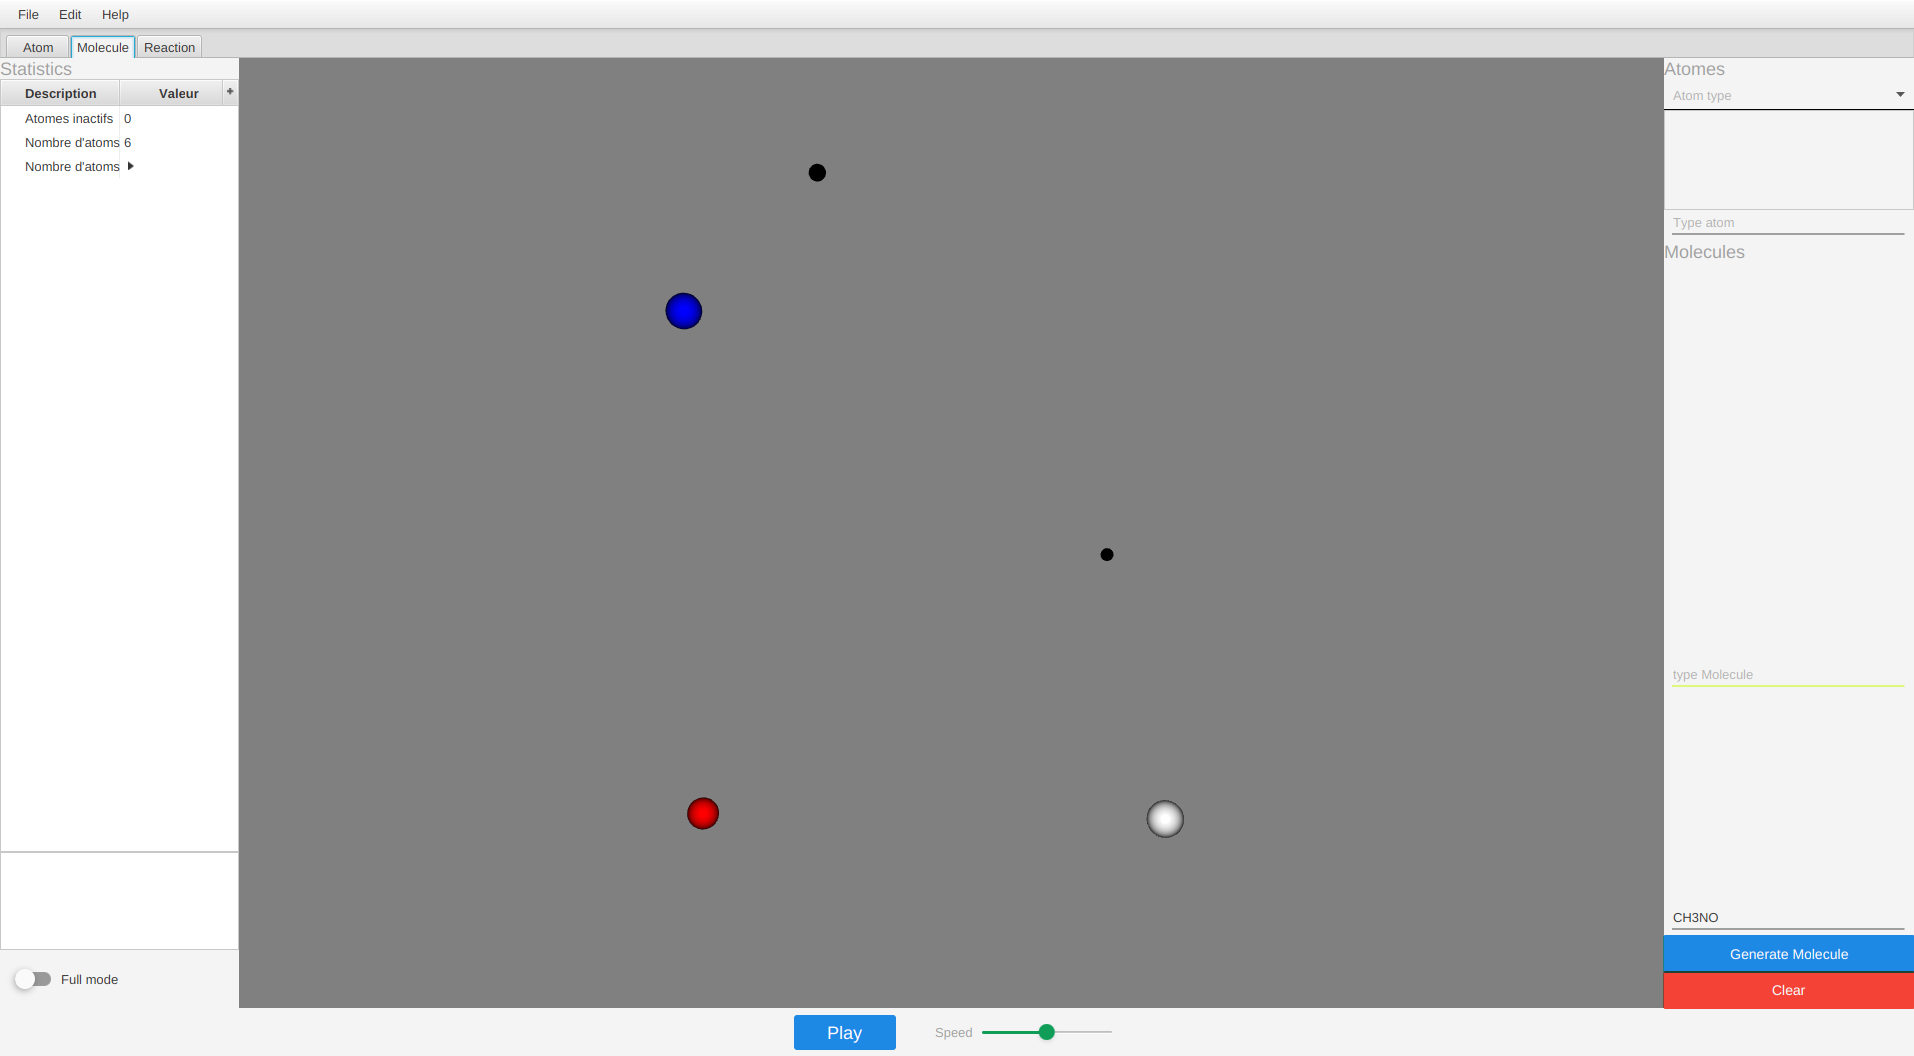
\includegraphics[width=1.2\textwidth]{screenshot_molecule}}
\caption{Vue sur l'onglet Molécule}
\label{screenshot_molecule}
\end{figure}

\paragraph{}
La vue Molécule permet de générer une molécule depuis une formule et de la
visualiser.


\begin{figure}[H]
\centering
\centerline{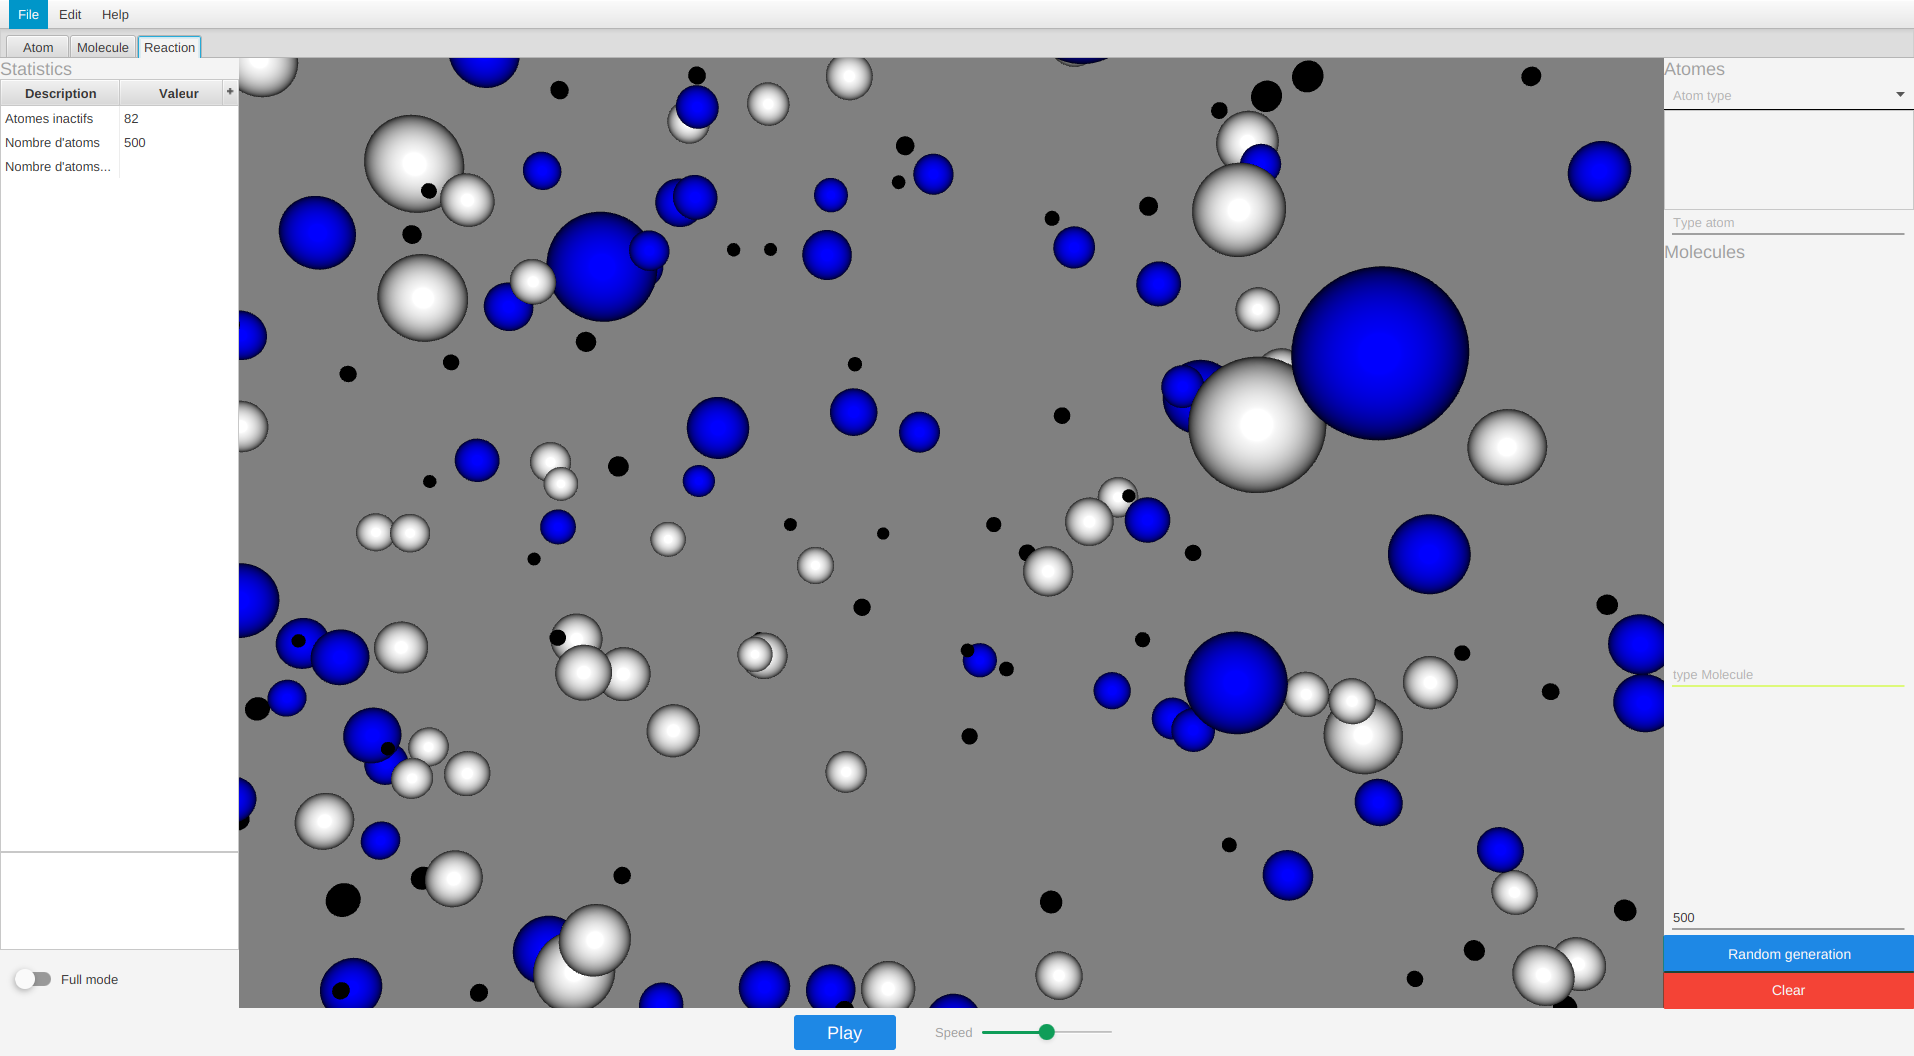
\includegraphics[width=1.2\textwidth]{screenshot_reaction}}
\caption{Vue sur l'onglet Réaction}
\label{screenshot_reaction}
\end{figure}

\paragraph{}
La vue réaction permet de générer un ensemble d'atomes, réagissant ensemble en
formant des molécules via un système d'attraction/répulsion.
